\chapter{Materials and Methods}
\section{Multiple Sequence Alignment}

Multiple sequence alignment (MSA) is an essential and well-studied fundamental problem in bioinformatics. It is used to compare and analyze the similarities between biological sequences. These sequences can be DNA, RNA, or protein sequences and can come from various species or different regions of the same genome. By aligning the sequences, it is possible to identify conserved regions that are important for the biological function or for evolution, as well as unique features that differentiate the sequences. Technically, alignments are generated and analyzed with computational algorithms. Fig.~\ref{FIG1} presents a sample (residue 1 to X) of the alignment results of the 25 sequences of GST studied in the present work. 

\begin{figure}[h!]
	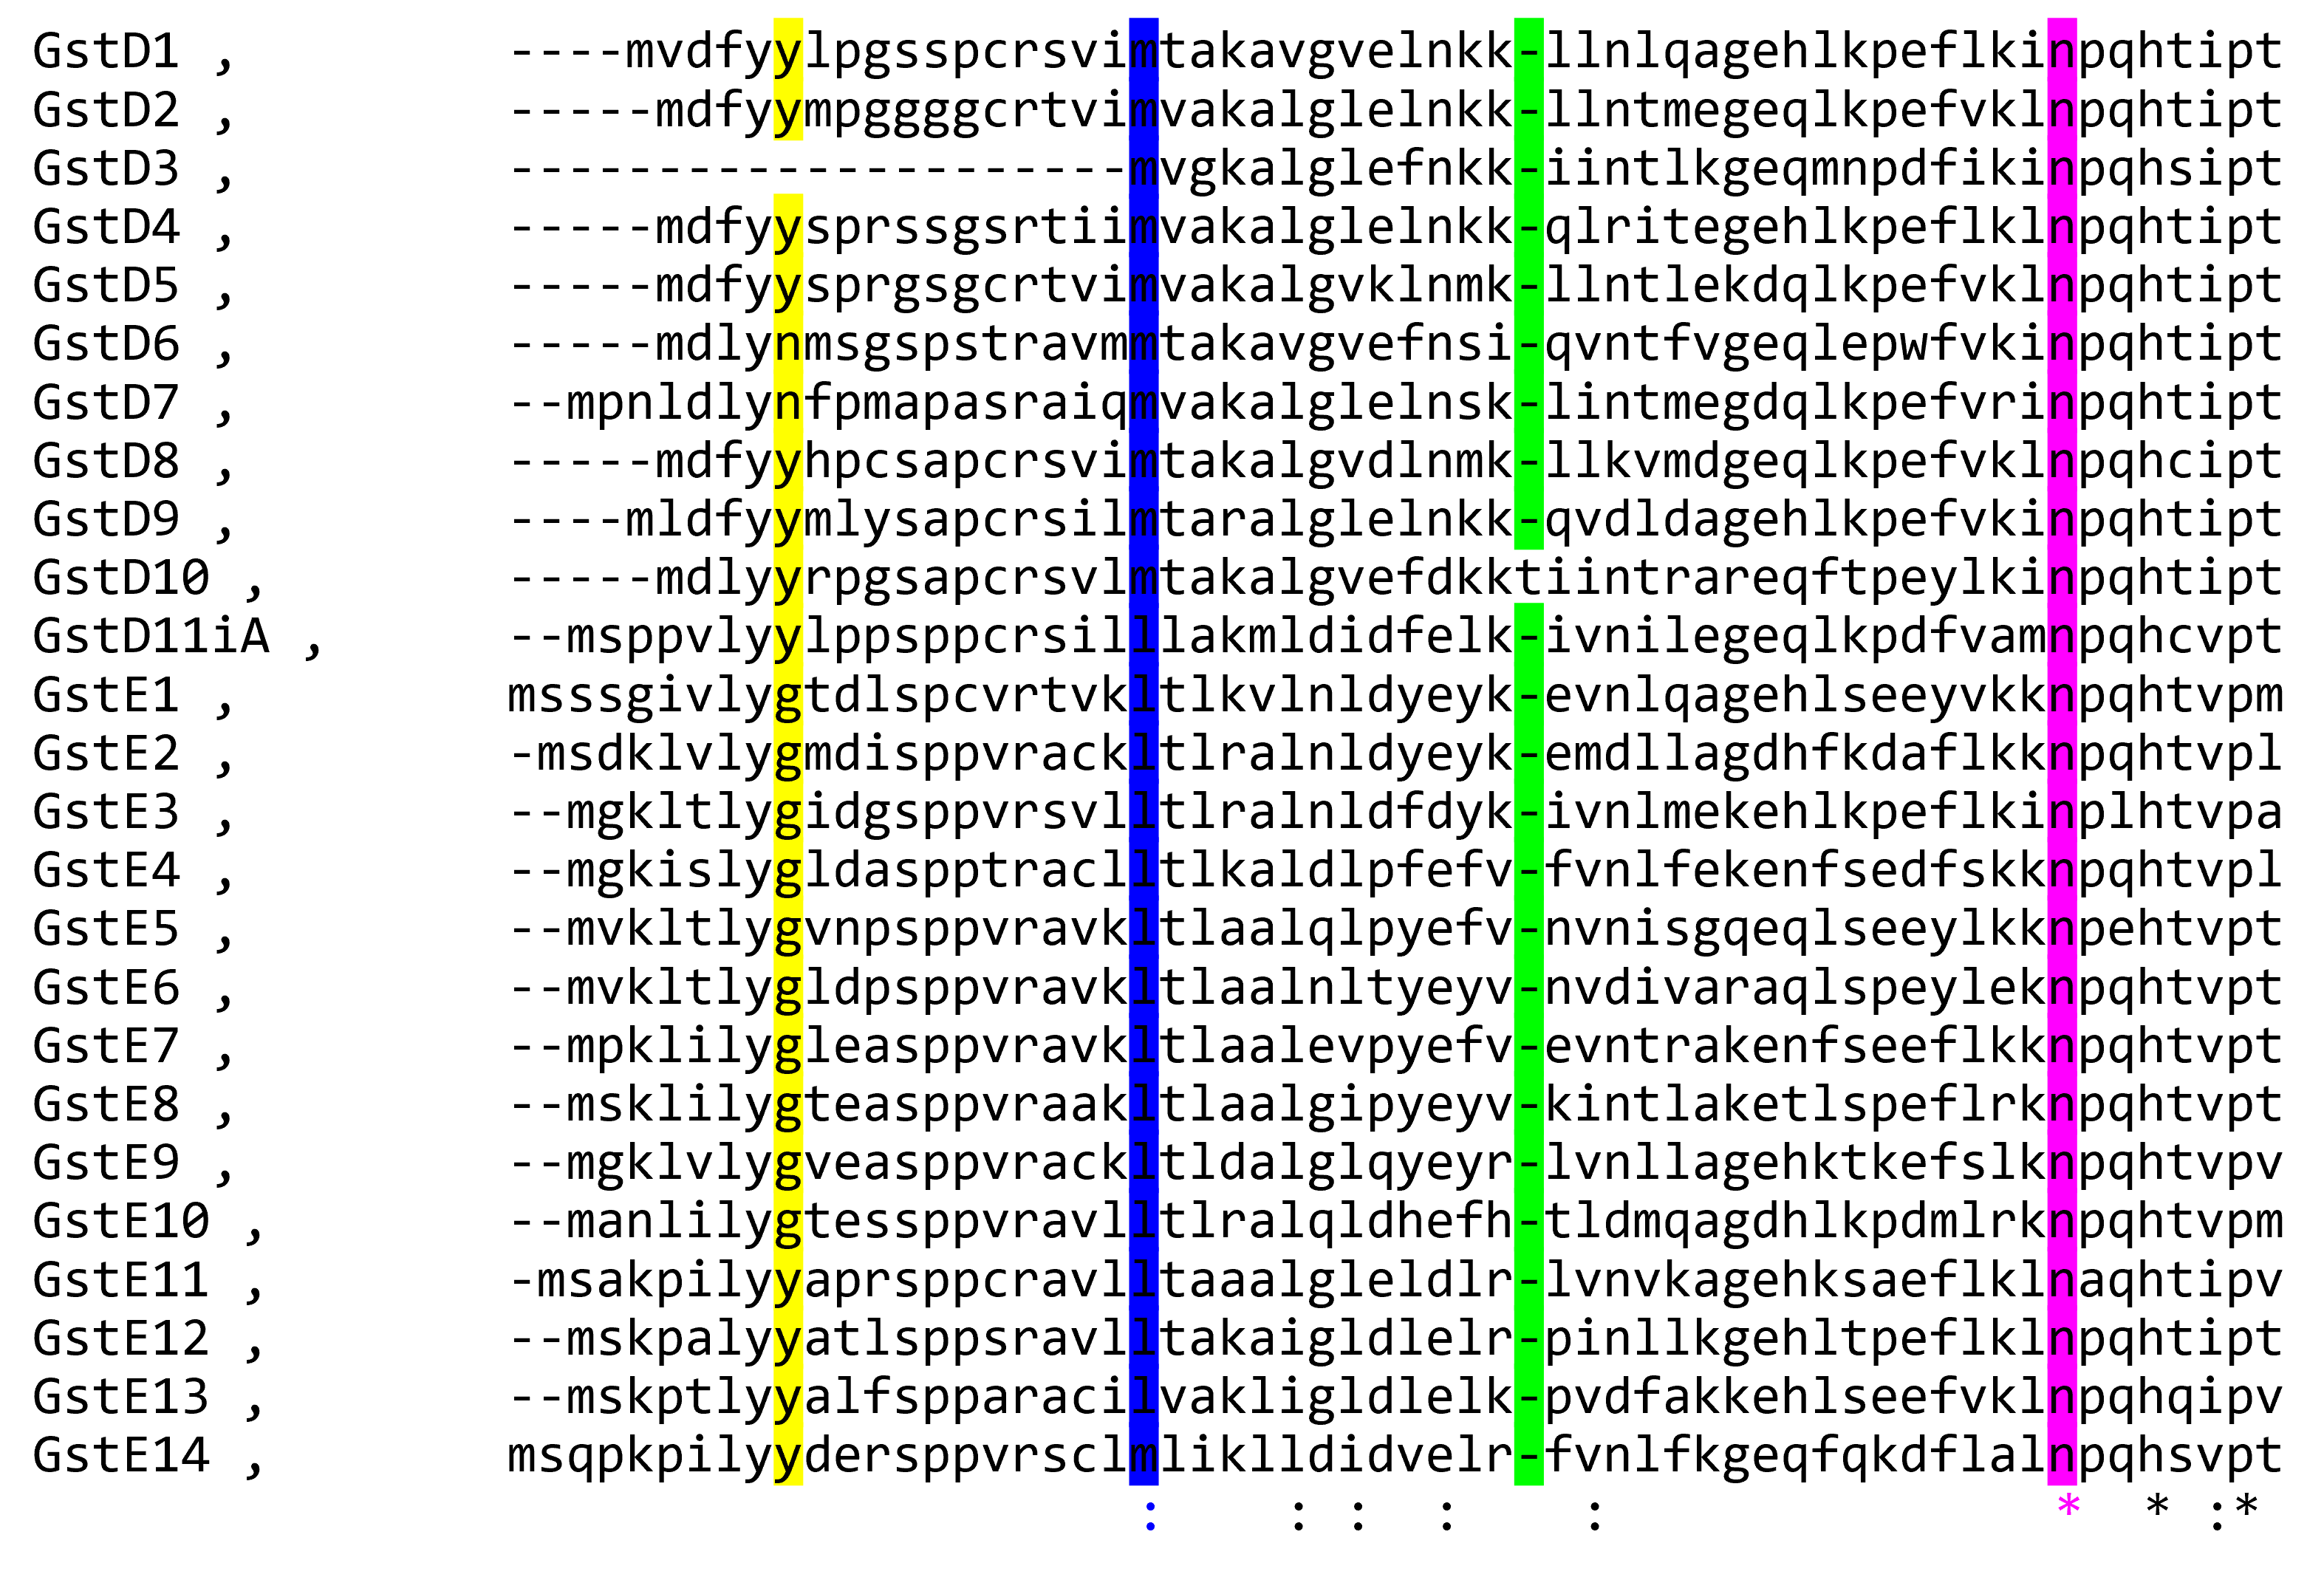
\includegraphics[width=12cm]{figures/MSA_sample.png}
	\caption{Sample of a Multiple Sequence Alignment applied to the 25 structures of GST. The color code is the following: identical amino acids (magenta), conservative substitution (blue), non-conservative substitution (yellow), gap (green).}
	\label{FIG1}
\end{figure}

Each row is the sequence of one of the molecules entered into the alignment. In this case, the top row is the sequence of the GSTD1 protein, the second row is the sequence of GSTD2 protein, etc. where each vertical column represents the amino acid at a position in the sequence. Underneath the bottom row for each block is a symbolic conservation score. A (-) indicates a gap between the two sequences, this happens when the sequences are of different length which is the case here (from X to Y residues). A (*) indicates that the amino acid is the same for the sequences at that position. A (:) indicates the sequences have different amino acids at that position, but that the chemical properties of the different amino acids are pretty similar. When an amino acid is substituted by a very similar amino acid at a position in an alignment, we call it a conservative substitution. A blank space ( ) indicates that the amino acids are very different at that position. We call that a non-conservative substitution.
\begin{itemize}
	\item Conservative substitution: The replacement of an amino acid residue in one protein by one with similar chemical properties in another protein. For example, the replacement of serine (S) by threonine (T), or leucine (L) by isoleucine (I), are both considered conservative substitutions.
	\item Non-conservative substitution: The replacement of an amino acid residue in one protein by one with dissimilar chemical properties in another protein. For example, the negatively charged glutamate (D) amino acid has quite different properties from the small glycine (G) residue, so this is an example of a non-conservative substitution.
\end{itemize}

In the present, we focus our interest on the ensemble of the 25 GST sequences described in the Introduction. Each sequence has a different length, making the alignment process particularly useful to extract properties along the sequence at a given position for comparison purpose. The MSA was performed using the XXXXXXX program. Through the MSA, we aim to identify regions of conservation in the 25 GST sequences, particularly for amino acids involved in the binding sites (BSs) and the interface of dimerization (IoD), which are two regions of the GST proteins that are very important for the biological function (see section 3.3). 

\section{AlphaFold}

Basically, the AlphaFold program directly predicts the 3-D coordinates of all heavy atoms for a given protein using the primary amino-acid sequence and aligned sequences of homologues as input (Fig.~\ref{FIG1}). To do so, AlphaFold extracts data from two major databases, \textit{i.e.} genetic and structural datasets and uses novel neural network architectures and training procedures based on the evolutionary, physical and geometric constraints of protein structures. The architecture jointly embed Multiple Sequence Alignment (see section 2.1) and pairwise features (2-D arrays). Then, the data processed through a network comprised of two main stages, called Evoformer and Structure module. More details about AI architectures of these two networks can be found here~\cite{AlphaFold}.

\begin{figure}[h!]
	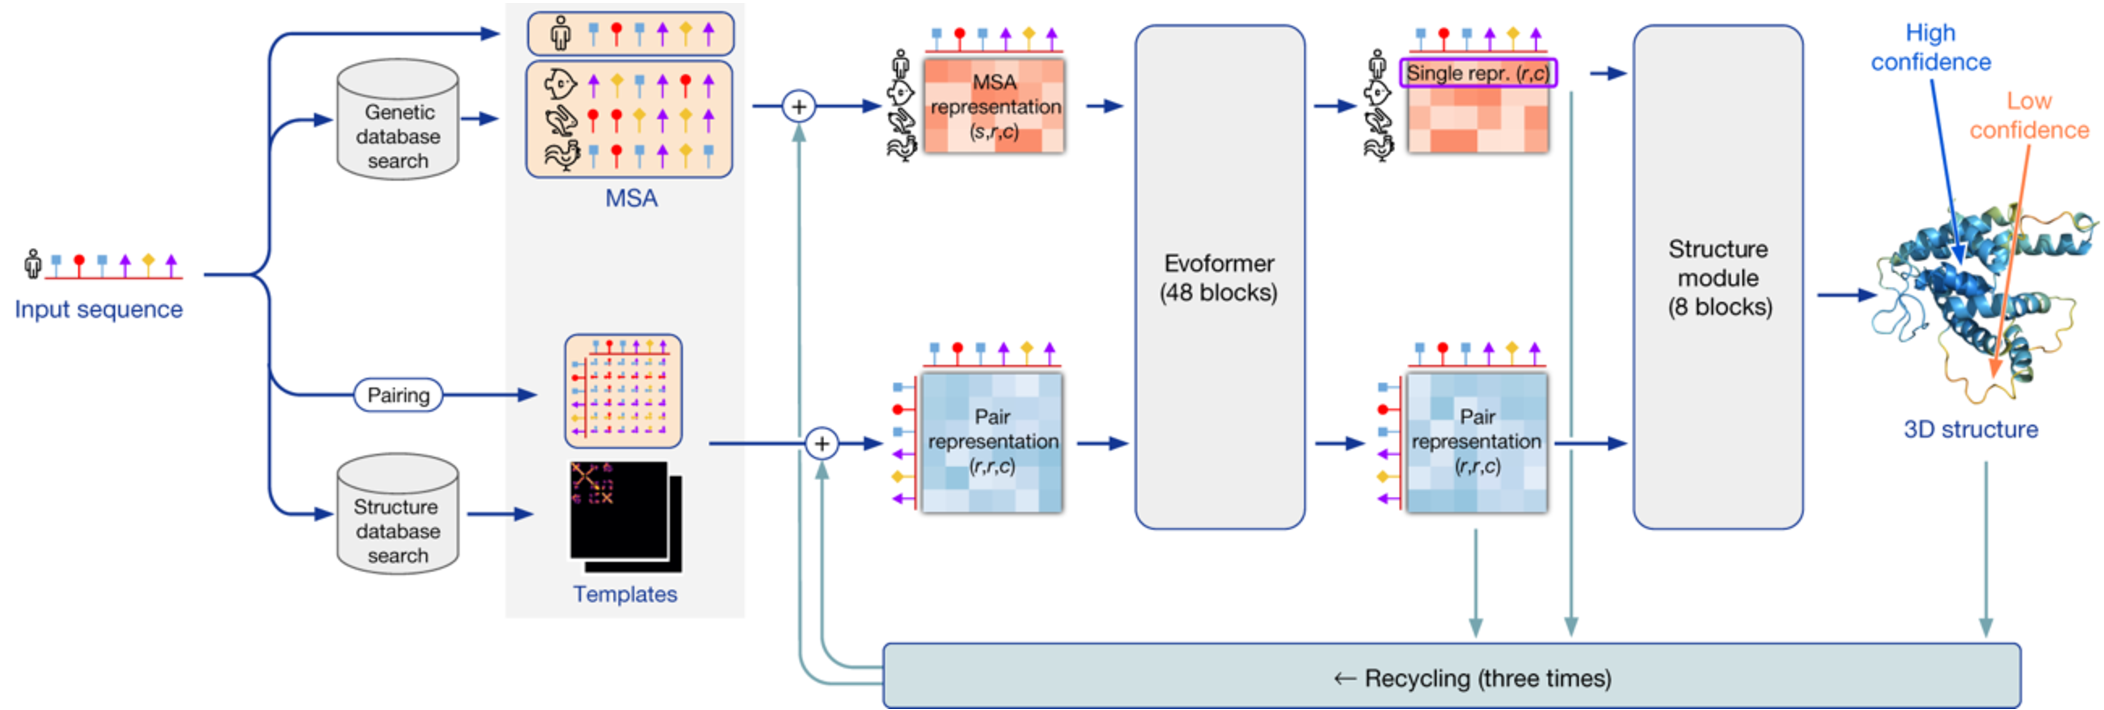
\includegraphics[width=16cm]{../figures/figure_AF_scheme.pdf}
	\caption{Model architecture of AlphaFold program. Arrows show the information flow among the various components. The figure was extracted from reference~\cite{AlphaFold}.}
	\label{FIG1}
\end{figure}

In the present work, we used the AlphaFold2-multimer program (add ref Mirdita M, Schütze K, Moriwaki Y, Heo L, Ovchinnikov S, Steinegger M. ColabFold: Making protein folding accessible to all. Nature Methods, 2022). The program implemented in Python (Jupyter Notebook) is available online:
\vspace{-1cm}
\begin{center}
	\bulurl{https://colab.research.google.com/github/sokrypton/ColabFold/blob/main/AlphaFold2.ipynb}
\end{center}

We used the default options, as already given in the Jupyter Notebook. At the end of the execution, the program proposes 5 different models of the 3-D structure of the protein and evaluates the predicted structures. Here, we consider only the best prediction available.

\section{Anisotropic Network Model}

The Anisotropic Network Model (ANM) is a simple yet powerful model made for Normal Mode Analysis of proteins, which has been successfully applied for deciphering the relationship between the biological function and the strucutral dynamics for many proteins\cite{ANM-COM}. In this model, the protein is represented as an elastic mass-and-spring network. In the network each node is the center of mass of the amino acid and the springs represent the interactions between the nodes. 

\begin{figure}[h!]
		%		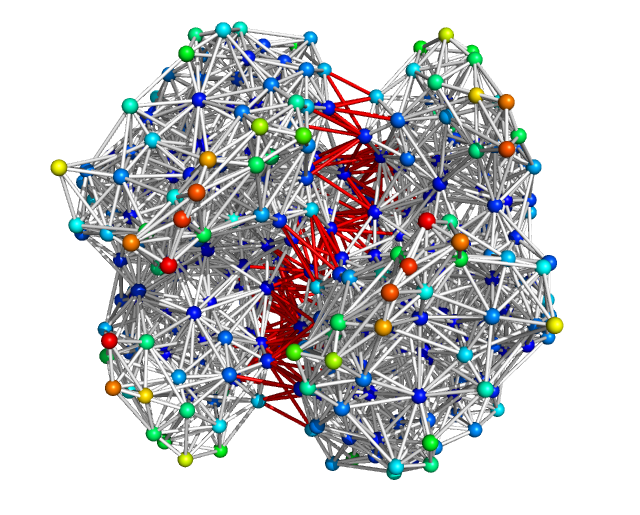
\includegraphics[width = .99\linewidth]{figures/GSTD1_ElasticNetwork.png}
	\caption{A) Cartoon representation of the GSTD1 protein. B) ANM representation of the GSTD1 protein as an elastic mass-and-spring network.}	
	\label{FIG2}
\end{figure}

\subsection{Theory}

The potential energy function is the sum of harmonic potentials between interacting nodes:
\begin{equation}
	V=\dfrac{\gamma}{2}\sum_{|R_{ij}^0|<R_c}(R_{ij}-R_{ij}^0)^2
\end{equation}
where $R_{ij}$ is the distance between atoms $i$ and $j$ and $R_{ij}^0$ is the distance between the atoms in the reference structure, e.g., the AlphaFold structure. The summation is only performed over atoms less than a cutoff distance $R_c$, and $\gamma$ is the force constant for the elastic bond between the atoms and is the same for all atoms pairs. In the Anisotropic Network Model, the mass-weighted Hessian matrix $\mathbf{\widehat{H}}$ for a network of $N$ nodes, derived from the second derivatives of the potential energy with respect to node positions, is of the form:
\begin{equation}
	\label{mass-weighted hessian matrix}
	\hat{H}_{ij} = -\gamma\dfrac{\Gamma_{ij}}{\sqrt{M_iM_j}}\cfrac{\vv{R_{ij}}\vv{R}_ {ij}^T}{R^2_ {ij}}
\end{equation}
where $\gamma$ is the spring constant used to model interactions between nodes, $M_i$ the mass of the node $i$ and $\Gamma$ is the contact matrix. In the case $i = j$, the force matrix is computed so that the self interacting term is the response to all the applied forces:
\begin{equation}
	\label{self interacting terms}
	\hat{H}_{ii} = -\sum_{j \ne i}\hat{H}_{ij}
\end{equation}
The normal modes are obtained by diagonalyzingn of the mass-weighted Hessian matrix:
\begin{equation}
	\label{eigen equation}
	\hat{H}\vv{e}_k = \tilde{\omega}_k^2\vv{e}_k
\end{equation}
with $3N-6$ non eigenvalues $\omega_k$ and their corresponding eigenvectors $\vv{e}_k$.\\

From the eigenvalues and eigenvectors of the mass-weighted Hessian matrix, one can compute two metrics of interest which characterize the local and non-local flexibility of a protein: the local mean square fluctuations (MSF) of a node $i$ and the non-local mean square fluctuations (MSF) of a pair node $(i,j)$ as:

\begin{equation}
	\label{thermal B-factors}
	\sigma^2(\vv{R}_i) = k_BT\sum_{k=1}^{3N-6}\frac{1}{\tilde{\omega}_k^2} \cfrac{\vert\vv{e}_{k, i}\vert^2}{M_i}
\end{equation}
\begin{equation}
	\label{metric dij}
	\sigma^2 (\vv{R}_{ij}) = k_BT\sum_{k=1}^{3N-6} \frac{1}{\omega_k^2}\left( \frac{\vv{e}_{k, j}}{\sqrt{M_j}} - \frac{\vv{e}_{k, i}}{\sqrt{M_i}} \right)^2
\end{equation}

Note that the local MSF $\sigma^2(\vv{R}_i)$ can be measured experimentally using XRD. It corresponds to the thermal B-factors corresponding to:

\begin{equation}
	B_i=\dfrac{8\pi^2}{3}\sigma^2(\vv{R}_i)
\end{equation}

When available, we compared the predicted values of the thermal B-factors with XRD data by computing the Pearson correlation coefficient as:

\begin{equation}
	\label{pearsonr}
	\mathcal{R} = \cfrac{\displaystyle\sum_i (\beta_i - <\beta>_i)(B_i - <B>_i)}{\sqrt{\displaystyle\sum_i(\beta_i - <\beta>_i)^2}\sqrt{\displaystyle\sum_j(B_j - <B>_j)^2}}
\end{equation}
The values of $\mathcal{R}$ are between $-1$ and $1$ and gives the linear correlation between predicted and measured B-factors. A coefficient of $1$ is associated to a perfect correlation whereas a coefficient of $0$ means that there is basically no links between prediction and experiment. 

\subsection{Parameterization}

In the ANM, two parameters are needed, \textit{i.e.} the spring constant $\gamma$ and the cutoff distance $R_c$ in order to characterize properly the local and non-local flexibility (MSF) of the proteins. To compute the contact matrix $\Gamma$ in Eq.~(\ref{mass-weighted hessian matrix}) and given two nodes $i$ and $j$, we consider $\Gamma_{ij} = 1$ if the distance $\vert\vv{R}_{ij}\vert \leq R_c$. At large distances, the interactions between the nodes are supposed to be small if not null. Therefore, $R_c$ is supposed to be here as small as possible. Moreover, the first six eigenfrequencies of the mass-weighted Hessian matrix are supposed to be zero, corresponding to the three global translations and rotations. In the case where $R_c$ is too small, the number of zero eigenfrequencies is larger than six, with no physical justifications. Therefore, the parameterization of $R_c$ is achieved with the smallest value that gives exactly $6$ zero eigenfrequencies. 

From Eq.~(\ref{mass-weighted hessian matrix}), it appears that  $\gamma$ is just a scaling factor. It can be estimated by comparing thermal B-factors computed using ANM with the ones measures by XRD  using least squared methods.

\begin{figure}[h!]
	%\includegraphics[keyvals]{imagefile}
	\caption{Parametrization of the ANM applied to the GSTD1 structure.}
	\label{FIG3}	
\end{figure}

Fig. \ref{Rc param} shows the parameterization of the cutoff $R_c$ obtained for ANM applied to the GSTD1 protein. From panel B, we can see that for $R_c = 7.5\AA$, the eigenvalues for $k \ge 6$ are no longer zero.

Add something about gamma and one grap of B-factors,scaled to XRD.